\documentclass[%
 reprint,
%superscriptaddress,
%groupedaddress,
%unsortedaddress,
%runinaddress,
%frontmatterverbose, 
%preprint,
%showpacs,preprintnumbers,
%nofootinbib,
%nobibnotes,
%bibnotes,
 amsmath,amssymb,
 aps,
%pra,
%prb,
%rmp,
%prstab,
%prstper,
%floatfix,
]{revtex4-2}

\usepackage{graphicx}% Include figure files
\usepackage{dcolumn}% Align table columns on decimal point
\usepackage{bm}% bold math
%\usepackage{hyperref}% add hypertext capabilities
%\usepackage[mathlines]{lineno}% Enable numbering of text and display math
%\linenumbers\relax % Commence numbering lines

%\usepackage[showframe,%Uncomment any one of the following lines to test 
%%scale=0.7, marginratio={1:1, 2:3}, ignoreall,% default settings
%%text={7in,10in},centering,
%%margin=1.5in,
%%total={6.5in,8.75in}, top=1.2in, left=0.9in, includefoot,
%%height=10in,a5paper,hmargin={3cm,0.8in},
%]{geometry}

%% Added by me: this forces the table caption to be on top.
\usepackage{lipsum}
\usepackage{hyperref}
\usepackage{floatrow}
\usepackage{gensymb}
\usepackage[thinc]{esdiff}
\floatsetup[table]{capposition=top}
\usepackage{listings}
\usepackage{color}

\definecolor{dkgreen}{rgb}{0,0.6,0}
\definecolor{gray}{rgb}{0.5,0.5,0.5}
\definecolor{mauve}{rgb}{0.58,0,0.82}

\lstset{frame=tb,
  language=Python,
  aboveskip=3mm,
  belowskip=3mm,
  showstringspaces=false,
  columns=flexible,
  basicstyle={\small\ttfamily},
  numbers=none,
  numberstyle=\tiny\color{gray},
  keywordstyle=\color{blue},
  commentstyle=\color{dkgreen},
  stringstyle=\color{mauve},
  breaklines=true,
  breakatwhitespace=true,
  tabsize=3
}

\begin{document}

\preprint{APS/123-QED}

\title{Generation and Analysis of Gas Particle Velocities \\from the Maxwell-Boltzmann Distribution}% Force line breaks with \\

\author{Neema Rafizadeh}
\altaffiliation[Email: ]{ rafizadehn@ku.edu}
\affiliation{%
Department of Physics and Astronomy, University of Kansas, Lawrence, KS, 66045, USA\\
% This line break forced with \textbackslash\textbackslash
}%

\date{\today}
%\date{\today}% It is always \today, today,
             %  but any date may be explicitly specified

\begin{abstract}

This experiment tested the ability for an apartment tenant to decide whether to trust their landlord about the furnace in their unit. To determine whether their apartment was actually a different temperature than the temperature outside, individual gas particles were sampled for their velocities and collected into a distribution. This was then compared to the null hypothesis and a statistical power analysis was performed. The number of particles was found to be less than 250 particles sampled to reach an 80\% confidence level in the ability to resolve the distributions. 
\end{abstract}


%\keywords{Suggested keywords}%Use showkeys class option if keyword
                              %display desired
\maketitle

%\tableofcontents

\section{Introduction \protect\\ }

Many physical systems studied in modern physics research follow the Maxwell-Boltzmann (M-B) distribution. From the study of electron diffusion in the semi-metal graphene to the modeling of photon interactions between a laser and a solid in photonics, the M-B distribution has proven to have great utility in explaining observed physical phenomena. The distribution has more fundamental roots in its derivation from the first principles of mass, temperature, and velocity of gas particles. However, the question becomes: how well can M-B curves truly be distinguished from one another?  

If there exists a room that has an unknown temperature, the M-B distribution can be used to experimentally determine its temperature by sampling particles from the gas in equilibrium in the room. The process of removing individual gas particles from a room and measuring its velocity by hand turns out to be quite arduous and taxing, thus determining the fewest number of particles that need to be sampled before a temperature can be determined is useful to know.

Take, for example, an apartment resident is told that their unit has an furnace set at 310 K while the temperature outside the building is 275 K. If the resident thinks their landlord is lying, they might want to determine if the furnace actually exists without access to it themselves. If they are able to measure the velocities of individual gas particles in the room, they can tell whether the conditioner is functioning by sampling the M-B distribution. The questions that they must consider become: \textit{are the possible temperatures too close to be distinguished experimentally?}\ and \textit{how many particles do we need to measure before we can tell them apart?}

Through probability statistics and power analysis, these questions can be answered and save people from countless hours of measuring velocities of gas particles by hand. Maybe this isn't a real problem. Oh well. Onward anyway\dots \textit{for science}.

\section{Hypotheses of Different Temperature Gases}

The M-B distribution is derived from basic physics principles based on some assumptions, namely that the gas particles are non-interacting, non-relativstic, and in thermal equilibrium. If this is the case, then the probability distribution that you find a particle with a particular velocity is given by,
\[
	f(m, v, T) = \left( \frac{m}{2\pi k T} \right)^{1/2}4\pi v^2 e^{-\frac{mv^2}{2kT}},
\]
where $m$ represents the molecular mass of the particles and $T$ represents the equilibrium temperature of the gas. Two examples of this probability distribution are plotted in Fig. 1 with temperatures 100 K and 1000 K. 

\begin{figure}[h]
	\caption{Probability density for gas particle velocity at differing temperatures, 100 k and 1000 K. Values taken for a gas with an 85 amu molecular mass. }
	\centering
	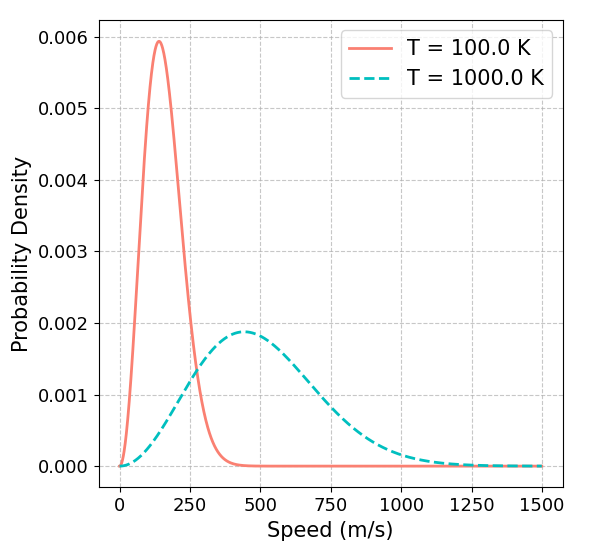
\includegraphics[scale=0.51]{hypothesis1.png}
\end{figure}

Note this is a probability \textit{density}, not a direct probability. Thus, the probability can be calculated through integration over a range of particle velocity. This means that the probability to find a particle at one particular velocity is 0 m/s as the integral will have the same two bounds of integration. Because of this, many statisticians plot cumulative density functions which represent the area under the curve of the probability density function up to a given value of velocity.

\section{Code and Experimental Simulation}

The plots in Fig. 1 are idealized curves that are plotted directly from the M-B distribution equation. To simulate a real experiment sampling gas particles, a random number generator is used in conjunction with the M-B equation and plotted as a histogram shown in Fig. 2. This is done by defining functions in python to return values of the M-B distribution, and also its inverse as shown in the listing below. From the \lstinline{rng_MaxBoltz.py} file,

\begin{lstlisting}
def boltz(v,m,T):
    kB = 1.38e-23
    return (m/(2*np.pi*kB*T))**1.5 * 4*np.pi * v**2 * np.exp(-m*v**2/(2*kB*T))

def inv_boltz(v,m,T):
    kB = 1.38e-23
    a = np.sqrt(kB*T/m)
    return erf(v/(np.sqrt(2)*a)) - np.sqrt(2/np.pi)* v* np.exp(-v**2/(2*a**2))/a
\end{lstlisting}
The M-B distribution takes physical parameters as an input and returns a probability density curve, while its inverse can give us the velocity values that we need to generate for the experiment. To get an entire distribution, another function can be defined to input arrays of randomly generated numbers to generate random velocities according to the M-B distribution.

\begin{lstlisting}
def velocities(n, seed):
    random = Random(seed)
    # rand_nums = np.random.rand(n)
    vals = []
    for i in range(0, n):
        vals.append(random.rand()
    )
    vel = inv_cdf(vals)
    return vel
\end{lstlisting}
This function requires use of the \lstinline{Random} class generated by Dr. Christopher Rogan and is available in his GitHub listed in Appendix A. 


\begin{figure}[h]
\caption{Histogram of particle velocities taken at a N = 1000 sample size. Values taken for a gas with an 85 amu molecular mass.}
\centering
	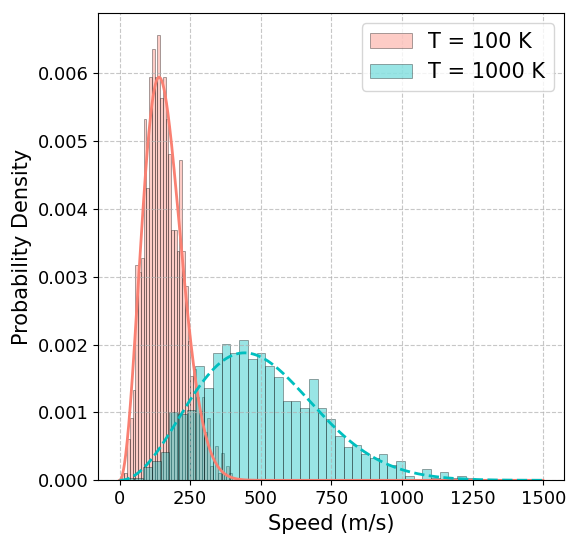
\includegraphics[scale=0.51]{code1}
\end{figure}

As seen in Fig.\ 2, the randomly generated velocity values closely resemble the idealized curves from before. See Appendix B to reference how the randomly generated velocities fit the idealized curves significantly better at a much higher sample size. The temperatures shown in Figs.\ 1 and 2 were chosen to be 100 K and 1000 K for demonstration, but this does not help the tenant in the apartment on the hunt for their elusive furnace. The temperatures used in the experiment are 275 K, which represents the null hypothesis (H$_0$), and 320 K, which represents our hypothesis we are testing against the null (H$_1$).

With temperatures so close together in value, it may not be as obvious to resolve the curves as it is with the 100 K and 1000 K curves. See Appendix C for a graphical representation of the 275 K and 320 K histograms next to one another. Instead of resolving our curves graphically, we will use a statistical power analysis to differentiate between the data we collect and the data from the null hypothesis. Through analysis of our type II errors (referred to as the value $\beta$), we can determine how often our data \textit{incorrectly} rejects the null hypothesis temperature, and then calculate our statistical power ($1-\beta$) from that. The statistical power is essentially the reverse of the type II error as it tells us how often we \textit{correctly} reject the null hypothesis. The higher the statistical power, the easier it is to distinguish data from the two temperatures, and thus the easier it will be for the apartment tenant to determine whether his landlord is juking him with his furnace. The calculation of this statistical power is given by the listing below.

\begin{lstlisting}
for i in percentiles:
	vel1_temp = vel1[0:int(i*N)]
	vel2_temp = vel2[0:int(i*N)]
	sp_temp = PSD(vel1_temp, vel2_temp)
	cd_temp = (np.mean(vel2_temp)-np.mean(vel1_temp))/sp_temp
	statistical_power = tt_ind_solve_power(effect_size=cd_temp, nobs1=len(vel1_temp), alpha=aval, ratio=1.0, alternative='two-sided')
	power.append(statistical_power)``
\end{lstlisting}
This section of code uses a python package named \lstinline{statsmodels} to calculate the log-likelihood ratios and uses it to calculate the power of the distributions. See Appendix A for more information regarding this package. It then appends it into an empty array named \textit{power} for each iteration of the gas particles sampled.

\section{Results and Analysis}

The results of this method are shown in Fig. 3 for 320 K, but also for other temperatures in the range of 290-330 K.

\begin{figure}[h]
	\caption{Statistical power plotted as a function of sample size. Values calculated with an $\alpha = 0.05$ value, and a molecular mass of 85 amu.}
	\centering
	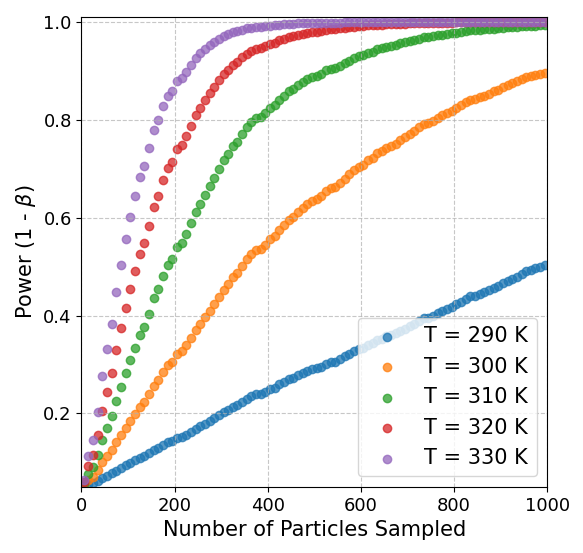
\includegraphics[scale=0.51]{results1.png}
\end{figure}

The different temperatures in Fig.\ 3 show the difference in statistical power per sample size in comparison to the other temperatures. Statisticians generally regard 0.8 to be a statistical power significant enough to consider two distributions resolvable. Since the apartment tenant is trying to resolve a temperature of 320 K, they would need to sample roughly 250 particles before reaching the 80\% confidence level.

Since the ability to distinguish between different scenarios of temperature depends heavily on the number of particles sampled, it is important for the apartment tenant to determine a temperature in which it will become unfeasable to distinguish between the distributions. They must then ensure the furnace is set outside of that range if they decide to pursue this experiment again. 

This makes intuitive sense as if the distribution is farther away from the null hypothesis, the tenant is more likely to pick a particle that does not fall within the range of the null hypothesis and determine quickly that they are able to reject it. For a temperature very close to the temperature of the null hypothesis, 275 K, it will require many more sampled particles before the tenant can confidently say they have a working furnace. This is demonstrated by the trend shown in Fig. 3 by the difference between the 290 K curve and the 330 K curve. 

\section{Conclusion}

A random number generator was used to sample velocity values from the Maxwell-Boltzmann distribution with a temperature parameter of 275 K and plotted into a histogram. Using this as the null hypothesis for the experiment, gas particles from the air were sampled from an apartment complex unit and compared against the null hypothesis to determine whether the complex had provided a furnace for the unit. The statistical power was calculated for different amount of sampled particles and a confidence level was found that could be used to determine the state of the furnace in the complex.

The temperature of 320 K is far enough away from the temperature outside of the apartment (275 K) that the tenant of the apartment was be able to tell the landlord was not lying to them at a 80\% confidence level from the 225 particles they measured. Through the use of statistical power analysis, the two distributions were able to be resolved from one another quite well despite the temperatures being so close in value. If the temperature values were closer, many more particles would need have been sampled before reaching the same 80\% confidence level used by the tenant in their experiment. 

In the future, this distribution can be studied further by changing other parameters of the M-B distribution. This may include things such as the mass or exploring similar distributions that do not have the same assumptions in their derivation from first princples. 

\acknowledgements

I would like to thank Prof.\ Chris Rogan for his continued support in the course. I would also like to thank Gbenga Agunbiade who assisted me with his peer review.

\appendix
\section{Sources and Raw Data}

All python scripts and data generated are contained in \href{https://github.com/rafizadehn/PHSX815_Project1}{\textcolor{blue}{Neema Rafizadeh's GitHub repository for this project}}. Instructions for running the scripts and changing the inputs are listed on the README.md file listed in that repository. 

The \lstinline{MySort} and \lstinline{Random} classes of functions can be located at \href{https://github.com/crogan/PHSX815_Week2}{\textcolor{blue}{Prof.\ Christopher Rogan's GitHub}}. The information regarding the Maxwell-Boltzmann distribution was sourced from the \href{https://en.wikipedia.org/wiki/Maxwell%E2%80%93Boltzmann_distribution}{\textcolor{blue}{Wikipedia article discussing the subject.}} The calculation of the statistical power was done with the \lstinline{statsmodels} package in python, with the \href{https://www.statsmodels.org/dev/generated/statsmodels.stats.power.tt_ind_solve_power.html}{\textcolor{blue}{docuentation provided here}}. 

\section{Histogram of Particle Velocities at Large Sample Size}

\begin{figure}[H]
	\caption{Histogram of randomly generated particles in a Maxwell-Boltzmann distribution. Number of particles generated is N = 100,000 particles ($10^5$).}
	\centering
	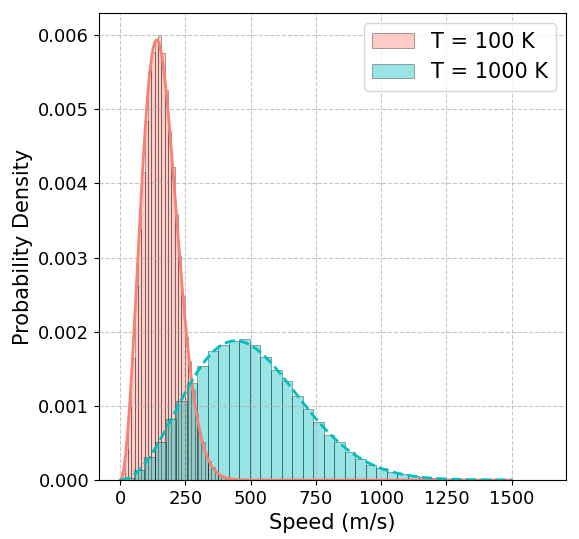
\includegraphics[scale=0.5]{appendix1.png}
\end{figure}

\section{Histogram of Particle Velocities at Simulated Scenario's Temperatures}

\begin{figure}[H]
	\caption{Probability density for gas particle velocity at differing temperatures, 275 k and 320 K. Values taken for a gas with an 85 amu molecular mass. }	
	\centering
	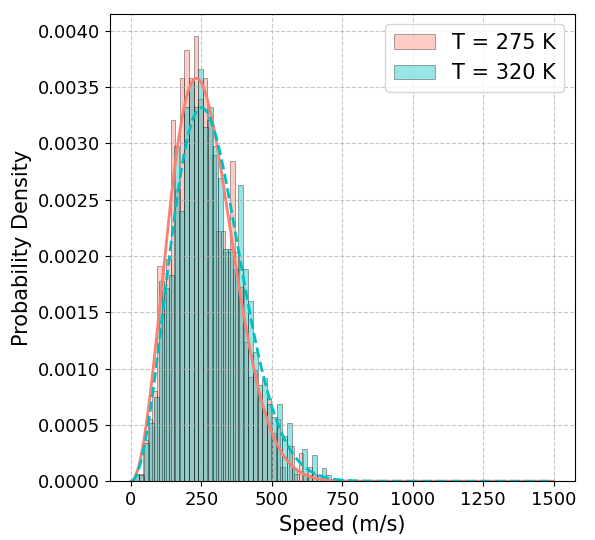
\includegraphics[scale=0.5]{appendix2.png}
\end{figure}

% The \nocite command causes all entries in a bibliography to be printed out
% whether or not they are actually referenced in the text. This is appropriate
% for the sample file to show the different styles of references, but authors
% most likely will not want to use it.
\nocite{*}

\bibliography{report_template}% Produces the bibliography via BibTeX.

\end{document}

%
% ****** End of file apssamp.tex ******
